\section{ Problem Statement/motivation}
%(like homework 1, what knowledge and how would you apply that knowledge, what is interesting that you hope to find)
 It is no secret that the new competition for this century is the 'hunt' for talents., "by 2030, more than 85 million jobs could go unfilled because there are not enough skilled people to take them, according to the latest study conducted by Korn Ferry."\footnote{ \url{https://www.kornferry.com/insights/this-week-in-leadership/talent-crunch-future-of-work}} "The shortage has been amplified by an insufficient number of U.S.-citizen computer science college graduates, restrictive (until recently) and limited H-1B visas for experienced IT professionals to fill the immediate gaps",  echoed the TechServe consulting. \footnote{ \url{https://www.techservealliance.org/news/the-state-of-the-technology-talent-shortage/}}
Dice.com's internal analysis already showed that we are going through technology workers (Technologists) shortage, and that is not due to the 'Great Resignation' but due to market demand. Our report will mine through the US H1B data set along with Dice.com's job and candidate profiles (along with skill sets for each job title),  to better understand which technologist job (e.g.: Software developer, Data scientist) are in increasing/decreasing demands, which skill sets (e.g.: Python, C++ etc.) are more popular/unpupular, through time-series. Our goal is to better understand the US technology market and what we can do to help people who try to get into tech market, by providing them with skill-set guidance along with professional training advice. \\
The motivation for this report came from a conversation with one product manager stating that there are no analysis on technologist supply and demand, even on salary data! The product analysts stated they don't have the data, and the R$\&$D team think it is a analyst job and should not 'waste' time on.  I decided to try that as a personal project. As I dive in more, I realized the official data set provided from department of labour is vague and uninformative, most of the job titles are lumped together, and focusing only on salary, hence no detailed information based on skills and locations. I then decided to mine other open source data, while adding relative skill set by mining seperate job description data set.\\
My philosophy to tackle this problem/project is to use a simple algorithm on multiple complicated sets, and not the other way: some complex algorithms  on a nice set instead. Personally, I had some 'fatigue' issues with words like 'Deep' and 'Neural' for now, both at work and school, so I've decided to do some old fashion mining by not using heavy GPU computing with 'sexy' machine learning titles, and just have some miner's fun with my hardhat and shovel.\footnote{I will leave that to CSCI 5922-Neural Networks and Deep Learning, this fall.}
\section{Literature survey}
SpaCy's Pipeline component for part-of-speech taggging\footnote{\url {https://spacy.io/api/tagger}} comes in  really handy for the  data preparation. What we did was to manually add a 'Tag' button for SMEs to spot the 'tech' words from our training set in HTML, resembling the following table:
{
	\begin{center}
		\begin{tabular}{| l | l | l | l | l | r| } 
			\hline
			&	Sentence	&	Word	&	Tag	 & POS &	Job description \# \\ \hline
			0	&	1	&	Softwares		&Tech	& NNPS	&description: 1 \\ \hline
			1	&	2	&	SQL	&	Tech	& NNP &	description: 1 \\ \hline
			2	&	3	&	Java	&	Tech & NNPJ	&	description: 1	\\ \hline
			3		&4		&Web	&	Tech	& NNS&	description: 1\\ \hline
			4	&	5	&	Azure		&Tech	& NNP	&description: 1\\ \hline
			\vdots	&		\vdots	&		\vdots		&	\vdots	&	\vdots	&	\vdots\\ \hline
		\end{tabular}
\end{center}}
Once we got enough samples, we apply the Viterbi algo to the future data set and mine the list of words for each job post, we then trim the list to get the overall skill-set for each title, like the following for sample job titles.  

\begin{center}
	\begin{tabular}{ | p{2.5cm} |p{4.5cm} |}
		\hline
		Job & Skills \\ \hline
		Net Application Developer& Microsoft technologies;Software development;C$\#$;HTML;Quality assurance;ASP.NET;Visual Basic .NET;.NET;Agile.\\\hline
		Android Developer	& Software development;Java;Mobile development;Quality assurance;Android development.\\\hline
		\vdots	&	\vdots\\ \hline
	\end{tabular}
\end{center}
\section{Proposed Work }
%E.g., what do you need to do for data collection, preprocessing (cleaning  integrating, transforming, etc.), process for derived data, design, evaluation. Describe how it is different than what has been done previously from your literature survey (or if replicating).
Shockly, the department of labour data does not give any insite on specific job title but a very general one. The following 3 code has most of the tech jobs: 
\begin{itemize}
	\item Management Occupations 11-0000
	\item Business and Financial Operations Occupations 13-0000
	\item Computer and Mathematical Occupations 15-0000
\end{itemize}
Roughly 35 of them instead of what we proposed of roughly 1400+. 
{\small {\begin{verbatim}
			
			['Computer and Mathematical Occupations',
			'Computer Occupations, All Other*',
			'Mathematical Science Occupations, All Other',
			'Computer Occupations',
			'Miscellaneous Computer Occupations',
			'Computer Occupations, All Other',
			'Mathematical Science Occupations',
			'Miscellaneous Mathematical Science Occupations',
			'Data Scientists and Mathematical Science Occupations, All Other'
			...
			]
\end{verbatim}}}
Which mean we either has to add a new attribute by clustering the 1400 into 15, or again write a new scrapper it mine glassdoor's data()This should not end up being a scrapper project), which does not guarentee accuracy since all are self-reported, which could be more biased than H1b data. Somehow, we have to reconcile that. 
\begin{itemize}
	\item Data scraping: Screaping HTML data from the web and store them in seperate json file
	\subitem EMPLOYER :  String, Nominal
	\subitem JOB TITLE :  String, Nominal
	\subitem BASE SALARY:  Float, Interval
	\subitem LOCATION:   String,  Nominal
	\subitem SUBMIT DATE:  (date) String, Ordinal
	\subitem START DATE:  (date) String, Ordinal
	\item Data cleaning: The most time consuming process, we need to be able to get rid of the outliers once we spotted them.
	\item Data preprocessing: Converting the saw data into meaningful use, for numeric data, we  need to convert them into float64, date has to be standard date type.
	\item Data integration: Integrate internal data with mined H1b data by join.
	\item Data mining and analysis: Clustering and time series. 
\end{itemize}
\section{Data set}
%(make sure you have the data set!). Provide URL and details about the data set (similar to homework 1, chapter 2, etc.)
\subsection{U.S. Department of Labor data}
What better resource to go to than the Department of Labor's statistics, After consulting with a product manger who points to the open API the department provided, I decide to mine their data first.  Shockly though, their data does not give any insight on specific job title but a very general one. I've choose to call the data between year 2010 and 2021 so that to better match with H1b's time series, and here's what we get, after thorough analysis  of 14027 data entries,with total 34 columns:\\
\begin{table}[h!]
	\caption{Deparrtment of  labour data }
	\resizebox{\columnwidth}{!}
	{%
		
		\begin{tabular}{llll}
			\hline
			{} &    count &  unique &                     top \\
			\hline
			occ\_code   &    14027 &    1507 &                 29-2010 \\
			occ\_group  &     9731 &       5 &                detailed \\
			occ\_title  &    14027 &    1272 &  Tour and Travel Guides \\
			group      &       46 &       2 &                   major \\
			tot\_emp    &  14027.0 &  8936.0 &                 11860.0 \\
			annual     &      852 &       1 &                    True \\
			hourly     &       62 &       1 &                    True \\
			year       &  14027.0 &     NaN &                     NaN \\
			area       &   2658.0 &     NaN &                     NaN \\
			area\_title &     2658 &       1 &                    U.S. \\
			prim\_state &     1329 &       1 &                      US \\
			emp\_prse   &  14027.0 &   229.0 &                     0.5 \\
			mean\_prse  &  14027.0 &     NaN &                     NaN \\
			a\_mean     &    14027 &    6155 &                       * \\
			a\_median   &    14027 &    5808 &                       \# \\
			\hline
		\end{tabular}
		
	}
\end{table}

There are 1272 job titles from department of labor open data, among  them, the only code (15-XXXX) that resemble our definition of technologist  is : 
\begin{itemize}
	\item Computer and Mathematical Occupations 15-0000
\end{itemize}
Unfortunately, only 37 of them instead  what we proposed of roughly 1400+ is publicly stored, they are:\\
{ \small
	\begin{itemize}
		\item 'Computer and Mathematical Occupations',
		\item	'Computer and Information Research Scientists',
		\item	'Computer Systems Analysts', 'Computer Programmers',
		\item	'Software Developers, Applications',
		\item	'Software Developers, Systems Software', 'Database Administrators',
		\item	'Network and Computer Systems Administrators*',
		\item	'Computer Support Specialists',
		\item	'Information Security Analysts, Web Developers, and Computer Network Architects',
		\item	'Computer Occupations, All Other*', 'Actuaries', 'Mathematicians',
		\item	'Operations Research Analysts', 'Statisticians',
		\item	'Mathematical Technicians',
		\item	'Mathematical Science Occupations, All Other',
		\item	'Computer Occupations', 'Computer and Information Analysts',
		\item	'Information Security Analysts',
		\item	'Software Developers and Programmers', 'Web Developers',
		\item	'Database and Systems Administrators and Network Architects',
		\item	'Network and Computer Systems Administrators',
		\item	'Computer Network Architects', 'Computer User Support Specialists',
		\item	'Computer Network Support Specialists',
		\item	'Miscellaneous Computer Occupations',
		\item	'Computer Occupations, All Other',
		\item	'Mathematical Science Occupations',
		\item	'Miscellaneous Mathematical Science Occupations',
		\item	'Database and Network Administrators and Architects',
		\item	'Database Administrators and Architects',
		\item	'Software and Web Developers, Programmers, and Testers',
		\item	'Software Developers and Software Quality Assurance Analysts and Testers',
		\item	'Web Developers and Digital Interface Designers',
		\item	'Data Scientists and Mathematical Science Occupations, All Other'.
	\end{itemize}
}

This dataset does not provide any details on what do these occupations include. We tried some online resources\footnote{\url{https://occupationdata.github.io/apst_mapping.pdf}} (including DoL's own mapping data from 2018\footnote{\url{https://www.bls.gov/soc/2018/home.htm}, only 20+ were able to  matched, that leaves 1380+ unmatched still }) to try mapping the 1400+ tech job into these 37 categories that yields horribly inaccurate result , which mean we either has to add a new attribute by clustering the 1400 into 15, or again write a new scrapper that mines Glassdoor's data (This should not end up being a scrapper project), even that does not guarantee a good  accuracy since all are self-reported, hence  more biased than H1b data. Due to the time limit, we have to reconcile that. 
\subsection{Scrapped H1b data}
{%
	\begin{table*}[h]
		\caption{Scrapped data as off July 15th}
		\begin{tabular}{llllllllll}
			\hline
			{} &   Dice\_job\_title &                           EMPLOYER &        JOB TITLE & BASE SALARY &      LOCATION & SUBMIT DATE &  START DATE &        Job\_Title  \\
			\hline
			count  &          2495079 &                            2495052 &          2467304 &     2467304 &       2467304 &     2467304 &     2467304 &          2495079  \\
			\hline
		\end{tabular}
	\end{table*}
}
\begin{itemize}
	\item 	H1B data  scraping from  from open data online.\footnote{\url{https://h1bdata.info/index.php}.}
	The data set is mainly from the United States Department of Labor (DOL) on how many H1-B petitions were filed and approved, with detailed information such as Employer, the title of  job, city/state locations, along with base salary,  submission and acceptance dates. 
	\item Skill set (Internal data)
	\item US Bureau of Labor Statistics \\
	\footnote{\url{https://www.bls.gov/developers/api$\_$python.htm}
	}
	\item Data mined and stored on my machine (Prcessor: 2.6 GHz 6-Core Intel Core i7. Memory: 32 GB 2667 MHz DDR4. Graphics:AMD Radeon Pro 5500M 4 GB
	Intel UHD Graphics 630 1536 MB).
\end{itemize}
\section{ Evaluation Methods }
%E.g., metrics, existing solutions, …\\
There are many ways how we can evaluate the results. Clustering Performance Evaluation Metrics like Silhouette coefficient is  a good start when applying clustering algorithm, for time series, all the error evaluations.  Besides, comparing time-series analysis data within each job we can compute the increaing or decreasing sides of each job along with correlations. Finally ,we are looking forward to apply all the relavent techniques we are currently learning in the class.\\
As for salary data, percentile based on title, location, and or starting time is definitely the first thing to try, $99\%$ and $1\%$ are definitely outliers for that, and balancing what percentile is something I need to be careful about. I am not thinking of 'elimination' since all data counts for that column, I may if it is way imbalanced. Hence we need separate analyses for both individuals and employers. For skill sets, I am considering density distance, which is yet to explore. Such as: 
\begin{figure}[h!]
	\begin{center}
		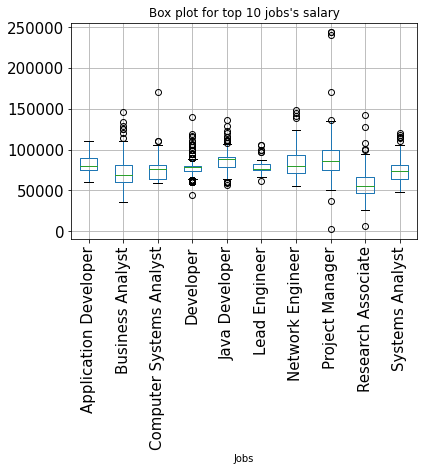
\includegraphics[width=.8\linewidth]{./photos/top10jobs.png}
	\end{center}
	\caption{Top 10 top job title with the highest pay boxplot.}
\end{figure}

\begin{figure}[h!]
	\begin{center}
		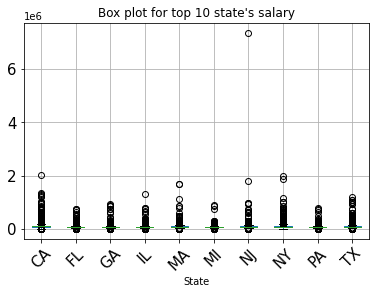
\includegraphics[width=\linewidth]{./photos/top10state.png}
	\end{center}
	\caption{Top 10 top state with the highest pay boxplot.}
\end{figure}
\subsection{Elbow method for clustering: TBD}
"Using the "elbow" or "knee of a curve" as a cutoff point is a common heuristic in mathematical optimization to choose a point where diminishing returns are no longer worth the additional cost. In clustering, this means one should choose a number of clusters so that adding another cluster doesn't give much better modeling of the data."\footnote{wikipedia}
\section{Tools}
\begin{itemize}
	\item Beautifulsoup for mining.
	\item Python library for all the computing and analysis.
	\subitem Spacy
	\subitem Sklearn 
	\subitem Tableau for visualization
	\item JSON for data store.
\end{itemize}
\section{Milestones Completed}

\begin{center}
	\begin{tabular}{ | p{2cm} |p{3.5cm} |p{2cm} |}
		\hline
		Date & Work Plan & Status\\ \hline
		Week 1 - 6: 16 May - 26 June& Research and data scrapping while class works. &Complete\\\hline
		Week 7: 27 June - 3 July & Submit Project Part 1: Project ProposalsAssignment.  &Complete\\\hline
		Week 8: 4 July - 10 July & Data cleaning  &Complete\\\hline
		Week 9: 11 July - 17 July & Submit Project Part 2: Proposal PaperAssignment  &Complete\\\hline
		Week 10: 18 July - 24 July & EDA and Classification Algorithms.  &semi-Complete \\\hline
	Week 10: 18 July - 24 July & Analyzing Department of Labor API data  &Complete \\\hline
	\end{tabular}
\end{center}

\section{Milestones to-do}
\begin{center}
	\begin{tabular}{ | p{2cm} |p{3.5cm} |p{2cm} |}
		\hline
		Date & Work Plan & Status\\ \hline
		Week 10: 18 July - 24 July & EDA and Classification Algorithms.  &semi-Complete \\\hline
		Week 11: 25 July - 31 July & Submit Project Part 3: Progress ReportAssignment. & Compelete\\\hline
		Week 12: 1 August - 7 August & Continue writing the project, and building interactive demo, build  an interactive Tableau dashboard. & To be Compeleted\\\hline
		(Final)Week 13: 1 8 August - 10 August & Submit Peer Evaluation Form, Project Final Report(with codes), and Project PresentationAssignment(Video).& To be Compeleted\\\hline
	\end{tabular}
\end{center}

%\section{Updated, extended version of initial proposal}
%\section{Proposal review: motivation, proposed work, tools, evaluation, milestones}
%\section{Milestones Completed: What you have achieved so far (in milestones section as a
%subtopic)}
%\section{Milestones Todo: What remains to be done (in milestones section as a subtopic)}
\section{Results so far } %(new topic at end)
%Any graphs, correlations, etc. if any
Although, the discovery does not mean DoL's data are completely worthless, there are some good insights that confirm our believe that tech talents are in rising demand. Take Figure \ref{dolnumofemployee} for example:
\begin{figure}[h]
	\begin{center}
		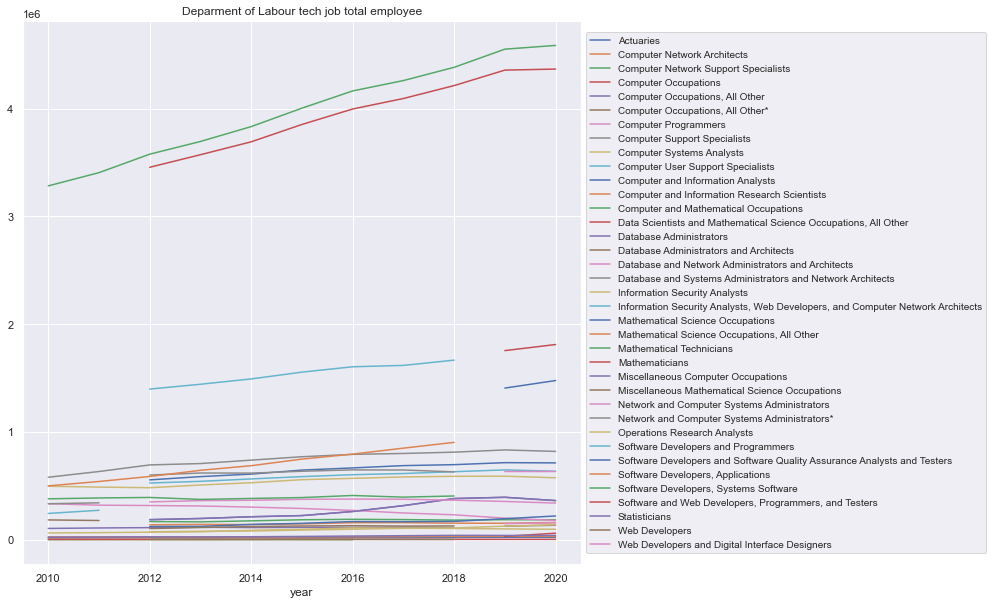
\includegraphics[width=\linewidth]{./photos/totaltech.png}
	\end{center}
	\caption{Deparment of Labour tech jobs number of employee.}
	\label{dolnumofemployee}
\end{figure}
The top 2 lines represent 'computer occupation' and 'software developer' professions, their growing rates are even higher than the rest of  technologists, it is a clear indication of higher demand for such labor, as opposed to the Farming jobs, which stays relatively the same, in some cases, even declined, as shown in Figure \ref{dolfarming}.
\begin{figure}[h]
	\begin{center}
		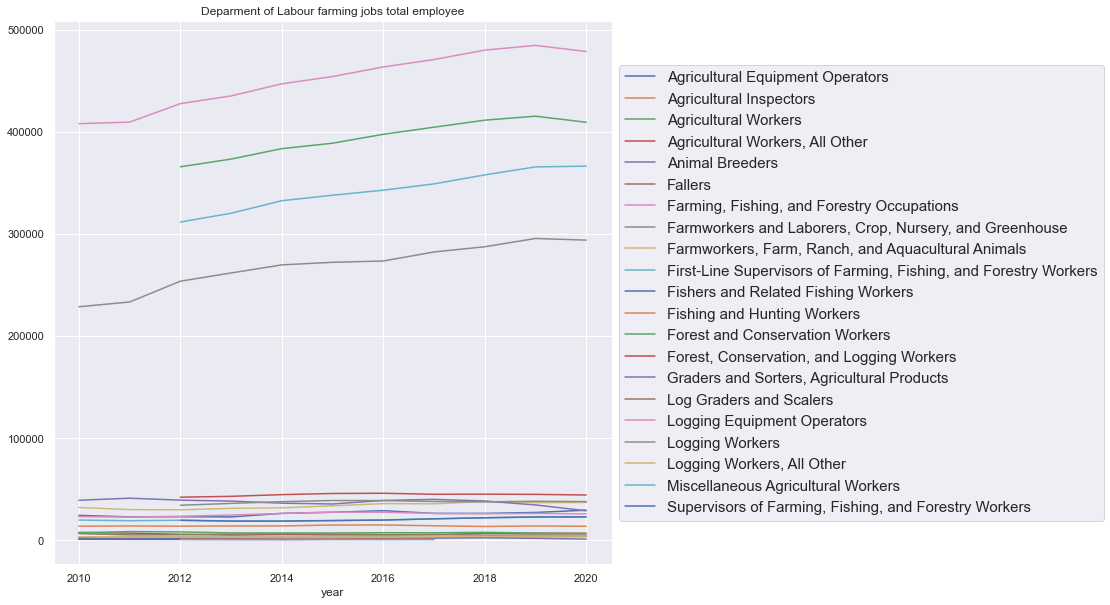
\includegraphics[width=\linewidth]{./photos/dolfarming.png}
	\end{center}
	\caption{Deparment of Labour farming jobs number of employee.}
	\label{dolfarming}
\end{figure}
If we look at the salary data for technologist in Figure \ref{techsalary}, we noticed the significant salary increase over the year, take into account the inflation and supply, it only amply the demand side of the tech market, which forces the employers to hand out competative salary. As oppose farming job market shown in Figure \ref{dolfarmingsalary}, where is did not even cover the inflation over a decade.
\begin{figure}[h]
	\begin{center}
		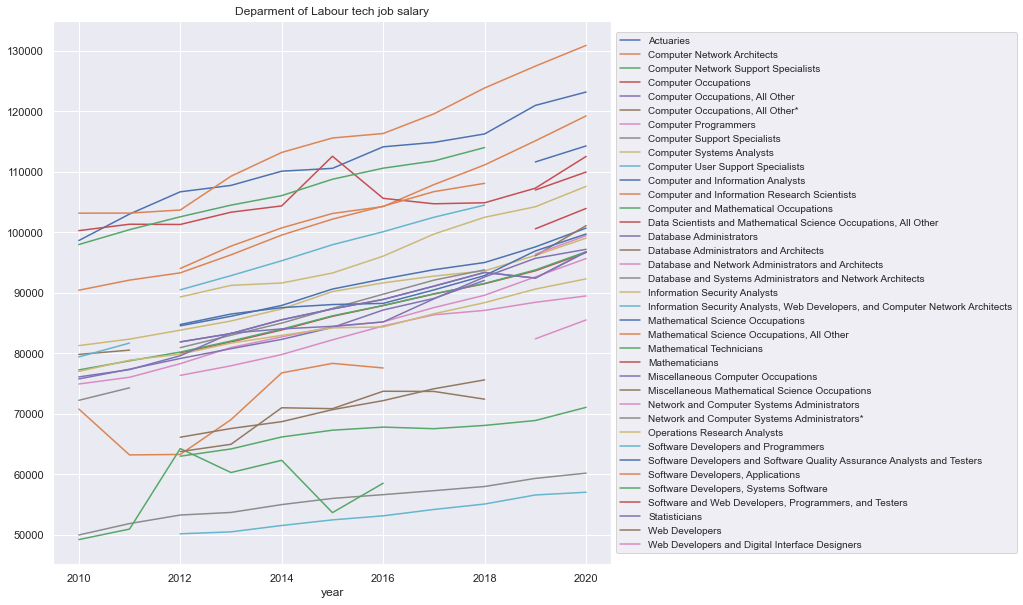
\includegraphics[width=\linewidth]{./photos/departmentoflabour.png}
	\end{center}
	\caption{Deparment of Labour tech job salary.}
	\label{techsalary}
\end{figure}

\begin{figure}[h]
	\begin{center}
		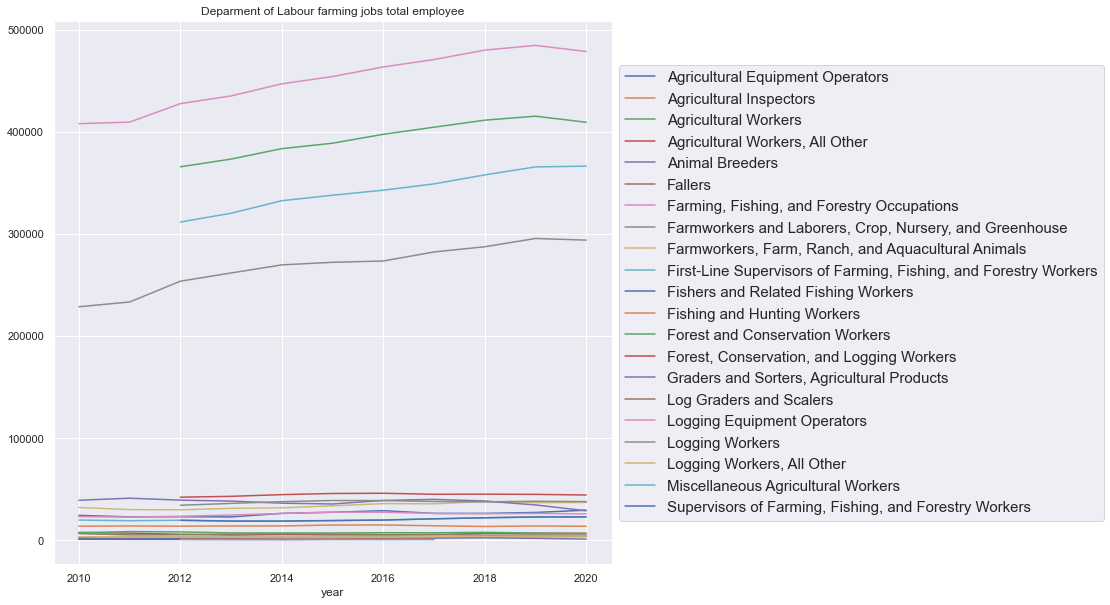
\includegraphics[width=\linewidth]{./photos/dolfarmingsalary.png}
	\end{center}
	\caption{Deparment of Labour farming jobs salary.}
	\label{dolfarmingsalary}
\end{figure}
All of these give us more reasons to find our own data, as an immigrant worker myself, the second 'gold mine' to dig is H1b, which will be the main focus of the next section.

\section{Part 1 Proposal feedbacks from classmates and my thoughts}
\subsection*{Pratik Prasanna Raghavendra}
Interesting topic, Abulitibu. Just curious, what would outlier data look like in your case? Also, how do you detect and eliminate them, since for example, really high income may simply be an outlier for individuals, but an important point for other employers?\\
My reply: As for salary data, percentile based on title, location, and or starting time is definitely the first thing to try, $99\%$ and $1\%$ are definitely outliers for that, and balancing what percentile is something I need to be careful about. I am not thinking of 'elimination' since all data counts for that column, I may if it is way imbalanced. Hence we need separate analyses for both individuals and employers.
For skill sets, I am thinking density distance, which is yet to be explored. 

\subsection*{Rohit Kharat}
I find this a unique topic and interesting to analyze in today's scenario. I liked that you are using web scraping, which I enjoy; using the BeautifulSoup library for web mining is fun. I am not familiar with the SpaCy library, something you can shed a light on. I also liked the idea of using location information for your analysis. I would recommend geolocation API something which I used earlier in my projects. I would also recommend doing feature reduction or getting the important features in your proposed work for focusing on only the crucial attributes. 
My reply: Seems like I need to reduce a lot of features. Too repetitive. The latest data shows:
\begin{table}[h!]

	\resizebox{\columnwidth}{!}
	{%
		
		\begin{tabular}{lllll}
			\hline
			{} &   count & unique &                                                top &   freq \\
			\hline
			Dice\_job\_title &  603967 &   1107 &                                    Systems Analyst &  35605 \\
			EMPLOYER       &  603967 &  66538 &                  TATA CONSULTANCY SERVICES LIMITED &  36885 \\
			JOB TITLE      &  603967 &   1655 &                                    SYSTEMS ANALYST &  35605 \\
			BASE SALARY    &  603967 &  37791 &                                             60,000 &  23256 \\
			LOCATION       &  603967 &  10453 &                                       NEW YORK, NY &  34957 \\
			SUBMIT DATE    &  603967 &   2747 &                                         03/16/2018 &   2377 \\
			START DATE     &  603967 &   2897 &                                         10/01/2020 &  17065 \\
			Job\_Title      &  603967 &   1107 &                                    Systems Analyst &  35605 \\
			relatedSkills  &  603967 &   1101 &  Software development;Systems analysis;SQL;Qual... &  35605 \\
			\hline
		\end{tabular}
		
	}
PCA is always my go to algorithm when I redecide to reduce the information's dimensions. For Geo, I think for now I will just use a really good map, since I still don't have demand data from job sites. 
\end{table}
\subsection*{Abhinav Gupta}
This looks like an unusual topic! Curious to see what your data cleaning and preprocessing would look like.
As your job skill data is internal, I don't know how it looks like, but I have a couple of questions. First question is that technologies are evolving and higher demand will always be for the new tech. As that tech, perhaps, is not even in the market yet, how would you predict the demand? Second question is if you would be considering countries and degrees as visa approval ratio varies highly on these factors. Final question is that as per uscis.gov - “The H-1B temporary visa program has been exploited and abused by employers primarily seeking to fill entry-level positions and reduce overall business costs”, so wouldn't your dataset be corrupted too?\\
My reply: For small or foreign companies, it seems sto be so, but not for big and advanced tech companies, Google filing counts for top 10, yet the salary is not below the market. It all depend on what we choose. I started as CPT then OPT, later H1b, yes, at first, I was the cheap labor, but once I accumulated enough skill, my salary is above the market while still on H1b, took almost 3 years. But when it comes to 'Corrupted' data, yes we do have that, and that's the purpose of introducing data mining, isn't it? 
\subsection*{Varun Manjunath}
An interesting topic. But is often the case that H1b workers are paid less as H1b is a nonimmigrant visa and is temporary in nature. So the point where you perform analysis on the dataset to check whether H1b workers are paid less is not very useful. Rather a more interesting trend would be to check which location hires the most H1b candidates. Dataset description with a bit more depth would be great in your case. Also, are you planning an inner join query to combine the datasets? Would suggest you remove certain outliers in the combined dataset before performing K-Means clustering.\\
My reply: left join mostly, inner join give few results.
\subsection*{Danielle Aras}
This is a very interesting and relevant topic. I agree that data cleaning is an important part of your project as you are merging different data sources with different features. I would be curious to know more details about the data sets like the size and date range. Technology is a fast moving field so the most current data will be the most useful for job seekers; looking at which jobs are trending up or down is a great idea.

I agree with other posters that the H1B visa data will introduce some challenges to your analysis. Given the trend of employers looking to take advantage of the system to under-pay workers, the popularity of H1B workers in a particular job may not actually correspond with a genuine demand that is not met by domestic workers. An interesting "spin-off" question would be creating an algorithm to detect companies abusing the system based on the availability of candidates in their area and H1B salaries.\\
My reply: I like this idea and will add it to discovery session.



